\documentclass[12pt,english]{article}
\usepackage[a4paper,bindingoffset=0.2in,%
            left=1in,right=1in,top=1in,bottom=1in,%
            footskip=.25in]{geometry}
\usepackage{amsfonts, amsmath, amssymb, physics}
\usepackage[utf8]{inputenc}
\usepackage[english]{babel}
\usepackage{indentfirst}
\usepackage[backend=biber, citestyle=nature]{biblatex}
\usepackage[nottoc]{tocbibind}
\usepackage{halloweenmath}
\usepackage{calligra}
\usepackage{esint}
\usepackage{graphicx}
\usepackage{hyperref}
\usepackage{xcolor}
\hypersetup{
  colorlinks   = true, %Colours links instead of ugly boxes
  urlcolor     = blue, %Colour for external hyperlinks
  linkcolor    = blue, %Colour of internal links
  citecolor   = red %Colour of citations
}
\usepackage{float}
\graphicspath{{./images/}}

%%%%%%%%%%%%%%%%%%%%% PREAMBLE %%%%%%%%%%%%%%%%%%%%%%%%
\setlength{\parindent}{2em}
\setlength{\parskip}{0em}

\newcommand{\dmr}[1]{\, \mathrm{d}#1} %command for the straight d (hehe)
\newcommand{\intt}[2]{\int_{#1}^{#2}} %easy integral command


\newtheorem{definition}{Definition}[section]
\newtheorem{theorem}{Theorem}[section]
\newtheorem{remark}{Remark}[subsubsection]

\numberwithin{equation}{subsection}

\addbibresource{ref.bib}


\DeclareMathAlphabet{\mathcalligra}{T1}{calligra}{m}{n}
\DeclareFontShape{T1}{calligra}{m}{n}{<->s*[2.3]callig15}{}
\newcommand{\curly}[1]{\ensuremath{\mathcalligra{#1}}}

\let\oldhat\hat
\renewcommand{\vec}[1]{\mathbf{#1}}
\renewcommand{\hat}[1]{\oldhat{\mathbf{#1}}}
\newcommand{\ar}[1]{\overset{\rightharpoonup}{#1}}
%%%%%%%%%%%%%%%%%%%%%%%%%%%%%%%%%%%%%%%%%%%%%%%%%%%%%%%

\title{PHYS2114 Cheat Sheet}
\date{June 2021}
\author{Joey Liang}

\begin{document}
\maketitle
\newpage
\tableofcontents
\newpage
\section{Mathematics Preliminary}
\subsection{IMPORTANT NOTE}
The following notations are taken from Griffths' `Introduction to Electromechanics'.\cite{Griffiths:611579}

Where as the line, area and volume integral elements are the following;
\begin{itemize}
    \item Line integral element: $\dmr{\vec{l}}.$
    \item Area integral element: $\dmr{\vec{a}}.$ 
    \item Volume integral element: $\dmr{\tau}.$
\end{itemize}

\par\noindent\rule{\textwidth}{0.4pt}

\subsection{Cartesian Coordinates}
The line and volume integral elements are
\begin{align*}
    \dmr{\vec{l}} &= \hat{x}\dmr{x} + \hat{y}\dmr{y} + \hat{z}\dmr{z}, & \dmr{\tau} = \dmr{x}\dmr{y}\dmr{z}.
\end{align*}

And the following are some common operators
\begin{align*}
    &\text{Gradient:} &\grad t  &= \pdv{t}{x}\hat{x} + \pdv{t}{y}\hat{y} + \pdv{t}{z}\hat{z},\\[1em]
    %
    &\text{Divergence:} &\grad\cdot\vec{v} &= \pdv{v_x}{x} + \pdv{v_y}{y} + \pdv{v_z}{z},\\[1em]
    %
    &\text{Curl:} &\grad \cross \vec{v} &= \left(\pdv{v_z}{y}-\pdv{v_y}{z}\right)\hat{x} + \left(\pdv{v_x}{z}-\pdv{v_z}{x}\right)\hat{y} + \left(\pdv{v_y}{x}-\pdv{v_x}{y}\right)\hat{z},\\[1em]
    %
    &\text{Laplacian:} &\laplacian t &= \pdv[2]{t}{x} + \pdv[2]{t}{y} +\pdv[2]{t}{z}. 
\end{align*}

\par\noindent\rule{\textwidth}{0.4pt}
\subsection{Cylindrical Coordinates}
The conversion of Cartesian to Cylindrical coordinates\cite{noauthor_cylindrical_2021} are 
\begin{align*}
    x &= r \cos \phi, & y &= r \sin\phi, & z &= z,
\end{align*}
note that $\phi \in [0,2\pi].$

And the surface integral element with radius $r$ constant is
\[
    \dmr{\vec{S}}    = r \dmr{\phi}\dmr{z}
\]    

The line and the volume integral elements are
\begin{align*}
    \dmr{\vec{l}} &= \hat{s}\dmr{s} + s\hat{\phi}\dmr{\phi}+\hat{z}\dmr{z}, & \dmr{\tau} = s\dmr{s}\dmr{\phi}\dmr{z}.
\end{align*}

The following are some common vector operators
\begin{align*}
    &\text{Gradient:} &\grad t  &= \pdv{t}{s}\hat{s}+\frac{1}{s}\pdv{t}{\phi}\hat{\phi}+\pdv{t}{z}\hat{z},\\[1em]
    %
    &\text{Divergence:} &\grad\cdot\vec{v} &= \frac{1}{s}\pdv{v_s}{s}(sv_s)+\frac{1}{s}\pdv{v_\phi}{\phi}+\pdv{v_z}{z},\\[1em]
    %
    &\text{Curl:} &\curl \vec{v} &= \left(\frac{1}{s} \pdv{v_z}{\phi} - \pdv{v_{\phi}}{z} \right)\hat{s} + \left(\pdv{v_{s}}{z} - \pdv{v_z}{s} \right)\hat{\phi} + \frac{1}{s}\left(\pdv{(s v_{\phi})}{s} - \pdv{v_s}{\phi}\right)\hat{z},\\[1em]
    %
    &\text{Laplacian:} &\laplacian t &= \frac{1}{s}\pdv{}{s}\left(s\pdv{t}{s}\right)+\frac{1}{s^2}\pdv[2]{t}{\phi}+\pdv[2]{t}{z}. 
\end{align*}
\par\noindent\rule{\textwidth}{0.4pt}

\subsection{Spherical Coordinates}
Note that $\theta\in[0,\pi]$ denotes the angle between z-axis and the vector of interest, and that $\phi\in[0, 2\pi]$ denotes the angle between x-axis and the projection of the vector of interest on to the xy-plane.\cite{noauthor_cylindrical_2021}

The conversion of Cartesian to Spherical coordinates are shown as the follows
\begin{align*}
    x &= r \sin(\theta)\cos(\phi), & y &= r \sin(\theta)\sin(\phi), & z &= r \cos(\theta).\\
\end{align*}

And the line and volume integral elements are
\begin{align*}
    \dmr{\vec{l}} &= \hat{r}\dmr{r} + r\hat{\theta}\dmr{\theta} + r  \sin(\theta) \hat{\phi} \dmr{\phi}, & \dmr{\tau} = r^2 \sin(\theta) \dmr{r} \dmr{\theta} \dmr{\phi}.
\end{align*}
with the surface integral with the radius $r$ constant is
\[
    \dmr{\vec{S}} = \sin\theta \dmr{\theta} \dmr{\phi}.
\]

The following are the common operators
\begin{align*}
    &\text{Gradient:} &\grad t  &= \hat{r}\pdv{t}{r} + \frac{\hat{\theta}}{r}\pdv{t}{\theta} + \frac{\hat{\phi}}{r \sin(\theta)}\pdv{t}{\phi},\\[1em]
    %
    &\text{Divergence:} &\grad\cdot\vec{v} &= \frac{1}{r^{2}} \frac{\partial}{\partial r}\left(r^{2} v_r \right)+\frac{1}{r \sin \theta} \frac{\partial}{\partial \theta}\left(v_{\theta} \sin \theta\right)+\frac{1}{r \sin \theta} \frac{\partial v_{\phi}}{\partial \phi},\\[1em]
    %
    &\text{Curl:} &\grad \cross \vec{v} &= \frac{1}{r\sin\theta}\left(\pdv{}{\theta}\sin(\theta) v_\phi- \pdv{v_\theta}{\phi}\right)\hat{r}\\
    &&&+\frac{1}{r}\left(\frac{1}{\sin\theta}\pdv{v_r}{\phi}-\pdv{}{r}  r v_\phi  \right)\hat{\theta}+ \frac{1}{r}\left(\pdv{}{r}rv_\theta-\pdv{v_r}{\theta}\right)\hat{\phi},\\[1em]
    %    
    &\text{Laplacian:} &\laplacian t &= \frac{1}{r^2}\pdv{}{r}\left(r^2\pdv{t}{r}\right)+ \frac{1}{r^2\sin\theta}\pdv{}{\theta}\left(\sin\theta\pdv{t}{\theta}\right) +\frac{1}{r^2 \sin^2 \theta}\pdv[2]{t}{\phi}.
\end{align*}

\par\noindent\rule{\textwidth}{0.4pt}

\subsection{Gauss' Divergence Theorem}
Suppose $V$ is a subset of $\mathbb{R}^n$ (in the case of $n=3$, $V$ represents a volume in three-dimensional space) which is compact and has a piecewise smooth boundary $S$ (also indicated with $\partial V = S$). If $\vec{F}$ is a continuously differentiable vector filed defined on a neighbourhood of $V$, then:
\[
    \iiint_{V} \left(\grad \cdot \vec{F}\right)\dmr{V} = \oiint_{S} \left(\vec{F}\cdot\hat{n}\right)\dmr{S}.
\]
\par The left side is a volume integral over the volume $V$, the right side is the surface integral over the boundary of the volume $V$. The closed manifold $\partial V$ is oriented by outward-pointing normal, and $\vec{n}$ is the outward pointing normal at each point on the boundary $\partial V$. ($\dmr{\vec{S}}$ may be used as a shorthand for $\vec{n}\dmr{S}$.) In terms of the intuitive description above, the left-hand side of the equation represents the total of the sources in the volume $V$, and the right-hand side represents the total flow across the boundary $S$.\cite{noauthor_divergence_2021}

\par\noindent\rule{\textwidth}{0.4pt}

\subsection{Stokes' Theorem}
Suppose we have a boundary $\partial \Sigma = S$ that bounds the surface $\Sigma$ with $\vec{F}$ defined in $\Sigma$, then
\[
    \iint_{\Sigma} (\grad \cross \vec{F})\cdot\vec{n}\dmr{S} = \oint_{S} \vec{F}\cdot \dmr{\vec{l}}.
\] 
\begin{figure}[h]
    \centering
    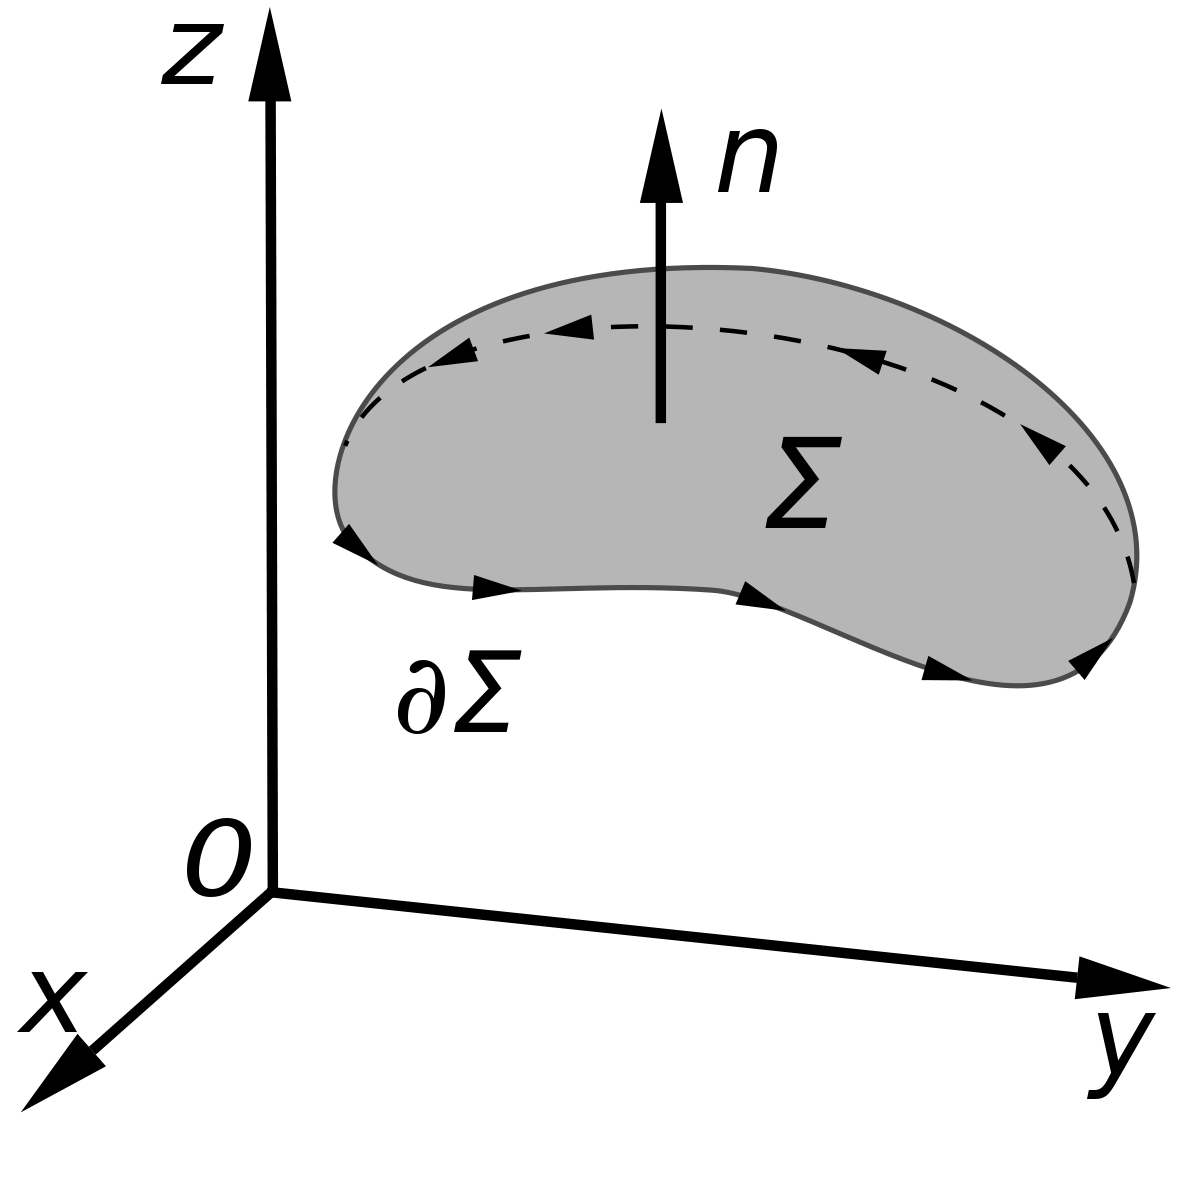
\includegraphics[width =0.5\textwidth]{1200px-Stokes'_Theorem.svg.png}
    \caption{A visual representation for the Stokes' theorem\cite{noauthor_stokes_2021}}
\end{figure}

\par\noindent\rule{\textwidth}{0.4pt}
\par\noindent\rule{\textwidth}{0.4pt}
\section{Electrostatics}
\subsection{The Holy Trinity}
\begin{align}
    &V = \frac{1}{4\pi\varepsilon_0}\iiint_{\mathcal{V}} \frac{\rho}{\curly{r}}\dmr{\tau}\\[1em]
    %%
    &\laplacian V = -\frac{\rho}{\varepsilon_0}\\[1em]
    %%
    &E = - \grad V\\[1em]
    %%
    &V = -\int \vec{E}\cdot \dmr{\vec{l}}\\[1em]
    %%
    &\vec{E} = \frac{1}{4\pi\varepsilon_0}\iiint_{\mathcal{V}} \frac{\hat{\curly{r}}}{\curly{r}^2}\rho\dmr{\tau}\\[1em]
    %%
    &\grad \cdot E = \frac{\rho}{\varepsilon_0}; \;\;\; \grad \cross E = 0
\end{align}
\begin{figure}[h]
    \centering
    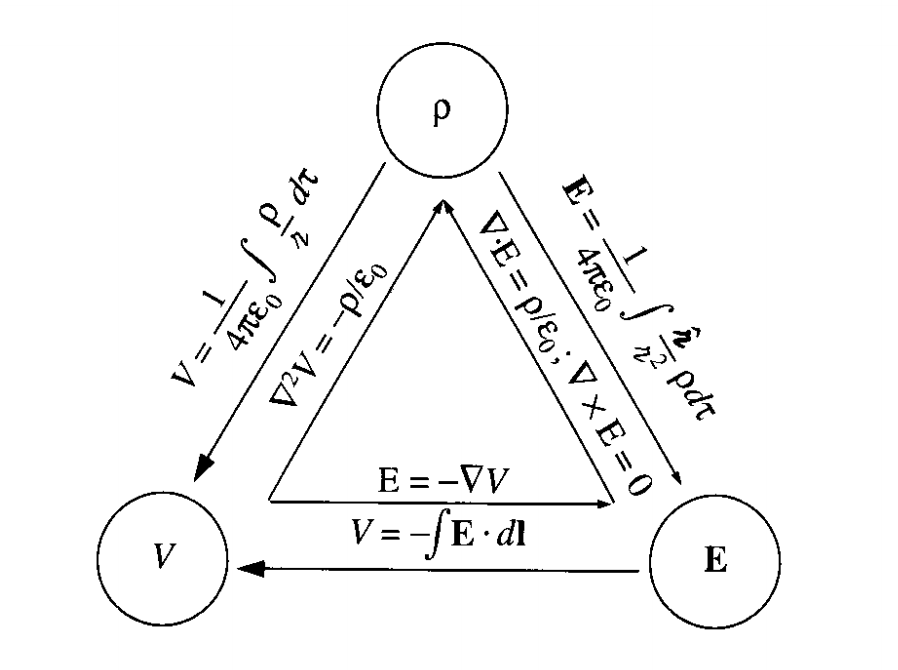
\includegraphics[width =0.5\textwidth]{holytrinity.png}
    \caption{The Griffith's holy trinity of electrostatics\cite{Griffiths:611579}}
\end{figure}

\par\noindent\rule{\textwidth}{0.4pt}
\subsection{Electrostatic Boundary Conditions}
\begin{align}
    \hat{n}_2 \cdot [\vec{E}_1-\vec{E}_2] &= \frac{\sigma}{\varepsilon_0}\\[0.5em]
    \hat{n}_2 \cross [\vec{E}_1-\vec{E}_2] &= 0\\[0.5em]
    V_1 - V_2 &= 0
\end{align}
Note that here the ``1" and ``2" just refer to the different sides of the interface.

\par\noindent\rule{\textwidth}{0.4pt}
\subsection{Work and Energy in Electrostatics}
Three important equations for Energy in work and energy in electro statics:
\par For discrete charges that are not very closed together,
\begin{equation}
    W = \frac{1}{2} \sum_{i = 1}^{n}q_i V(\vec{r}_i).
\end{equation}
\par For volume charge density $\rho$, 
\begin{equation}
    W = \frac12 \iiint_{\mathcal{V}} \rho V \dmr{\tau}.
\end{equation}
\par And even more simply, we can have,
\begin{equation}
    W = \frac{\varepsilon_0}{2}\iiint_{\mathbb{R}^3}E^2\dmr{\tau}.
\end{equation}

\par\noindent\rule{\textwidth}{0.4pt}
\subsection{Conductors}
There are \textbf{five} fundamental properties of a conductors,
\begin{enumerate}
    \item $E = 0$ inside a conductor.
    \item $\rho = 0$ inside a conductor.
    \item Any net charge resides on the surface.
    \item A conductor is an equipotential.
    \item $E$ is perpendicular to the surface, just outside a conductor.
\end{enumerate}

Now, let's consider the force per unit area $\vec{f}$ on any charges that rests on the surface of the conductor, with references to page 102 in the book,\footnote{`The book' is exclusively used in this note to `Introduction to Electromagnetism' by David J. Griffths} we know that
\begin{equation}
    \vec{f} = \sigma \vec{E}_{\text{average}} = \frac12 \sigma (\vec{E}_{\text{above}}-\vec{E}_{\text{below}}).
\end{equation}
In particular, that for conductors, where we know $\vec{E}_{\text{below}} = 0$ (equipotential inside the conductor), we obtain 
\begin{equation}
    \vec{f} = \frac{1}{2\varepsilon_0}\sigma^2 \hat{n}
\end{equation} 
\par\noindent\rule{\textwidth}{0.4pt}

\subsection{Capacitors}
Note that the one thing we need to know about capacitance is that it is nothing but a ``proportionality" between the stored charge and the potential difference;
\begin{equation*}
    Q = CV.
\end{equation*}


\section{Special Techniques}
\subsection{Uniqueness Theorems}
\textbf{First uniqueness theorem:} The solution to Laplace's equation in some volume $\mathcal{V}$ is uniquely determined if $V$ is specified on the boundary surface $S$.

\textbf{Second uniqueness theorem:} In a volume $\mathcal{V}$ surrounded by conductors and containing a specified charge density $\rho$, the electric field is uniquely determined if the \textit{total charge} on each conductor is given. (The region as a whole can be bounded by another conductor, or else unbounded.)\cite{Griffiths:611579}
\par\noindent\rule{\textwidth}{0.4pt}
\subsection{Separation of Variables}
\subsubsection{Cylindrical Coordinate}
You can find the full derivation \href{http://faculty.washington.edu/blayneh/cylcoord.pdf}{\textbf{here.}} For those who just care about the result (of potential $V$) without $\hat{z}$ dependence
\begin{multline}
    V(s,\phi) = a_0 + b_0 \ln s\\
    + \sum_{k=1}^{\infty} \left[ s^k ( a_k \cos k \phi + b_k \sin k \phi) + s^{-k} (c_k \cos k \phi + d_k \sin k \phi) \right].
\end{multline}

\subsubsection{Spherical Coordinate}
Once again, you can find the full derivation \href{http://www.physics.usu.edu/Wheeler/EM3600/Notes11SeparationOfVariablesSpherical.pdf}{\textbf{here.}} And the general result for the potential $V(s, \theta, \phi)$ is
\begin{equation}
    V(s, \theta, \phi) = \sum_{l = 0}^{\infty} \sum_{l}^{m=-l} \left(A_{lm}r^l + \frac{B_{lm}}{r^{l+1}} \right) P_{l}^{m}(\cos \theta) \exp(im\phi)
\end{equation}
\par\noindent\rule{\textwidth}{0.4pt}
\subsection{Multipole Expansion}
\subsubsection{The Multipole Expansion}
Note that $P_n$ represents the $n^{\text{th}}$ Legendre Polynomial,
\begin{equation}
    V(\vec{r})=\frac{1}{4\pi\varepsilon_0} \sum_{n=0}^{\infty}\frac{1}{r^{n+1}}\int(r')^{n}P_n(\cos \theta')\rho(\vec{r}')\dmr{\tau'}.
\end{equation}

\begin{figure}[H]
    \centering
    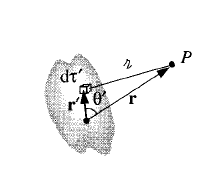
\includegraphics[width =0.5\textwidth]{multipole.png}
\end{figure}

\subsubsection{The Dipole Term}
Since $P_0 = 1$, the dipole moment is then 
\begin{equation}
    \vec{p} = \int \vec{r'} \rho(\vec{r'}) \dmr{\tau'}.
\end{equation}

And the dipole (DIPOLE ONLY) contribution to the potential is
\begin{equation}
    V_{\text{dip}}(\vec{r}) = \frac{1}{4 \pi \varepsilon_0} \frac{\vec{p}\cdot\hat{r}}{r^2}.
\end{equation}

\subsubsection{The Electric Filed of a Dipole}
The electric field is simply 
\begin{equation}
    \vec{E}_{\text{dip}}(r,\theta)=\frac{p}{4 \pi \varepsilon_0 r^3}(2\cos \theta \; \hat{r} + \sin \theta \; \hat{\boldsymbol\theta}).
\end{equation}




\par\noindent\rule{\textwidth}{0.4pt}
\par\noindent\rule{\textwidth}{0.4pt}
\section{Electric Field in Matter}

\subsection{Polarisation}
The torque a dipole experiences due to a field $\vec{E}$ is 
\begin{equation}
    \vec{N} = \vec{p} \cross \vec{E}.
\end{equation}
And the force the dipole experiences is 
\begin{equation}
    \vec{F} = (\vec{p}\cdot\vec{\nabla})\vec{E}
\end{equation}
\par\noindent\rule{\textwidth}{0.4pt}

\subsection{Induced Dipoles}
Suppose we have an uniform electric field $\vec{E}$, and an atom (dipole) is in this field. This atom will now posses some dipole moment. The dipole moment is \textbf{most of the times} approximately proportional to the field.
\begin{equation}
    \vec{p} = \alpha \vec{E}.
\end{equation}
\par\noindent\rule{\textwidth}{0.4pt}
\subsection{Bound Charges}
Let's suppose we have a blob of polarised material, with dipole moment $\vec{p} = \vec{P}(\vec{r'})\dmr{\tau'}$ in each volume element. The total potential is 
\[
    V(\vec{r})= \frac{1}{4 \pi \varepsilon_0}\iiint_{\mathcal{V}}\frac{\hat{\curly{r}}\cdot \vec{P}(\vec{r'})}{\curly{r}^2}\dmr{\tau'}.
\]
And after some maths, we then obtain
\begin{equation}
    V = \frac{1}{4 \pi \varepsilon_0} \oiint_{\mathcal{S}} \frac{1}{\curly{r}} \vec{P}\cdot \dmr{\vec{a'}} - \frac{1}{4 \pi \varepsilon_0} \iiint_{\mathcal{V}} \frac{1}{\curly{r}} (\grad \cdot \vec{P}) \dmr{\tau'}.    
\end{equation}

Notice that 
\begin{align*}
    \underbrace{\sigma_{b} = \vec{P} \cdot \hat{n}}_{\text{Surface bound charge}}, &&\text{and}&& \underbrace{\rho_b = -\grad \cdot \vec{P}}_{\text{Volume bound charge}}.
\end{align*}

Those are called bound charges (surface bound charges \& volume bound charge), we can just find them to get the voltage of the polarised dialectic blob instead of calculating the massive integral.
\par\noindent\rule{\textwidth}{0.4pt}
\subsection{The Electric Displacement}
\subsubsection{Gauss's Law in the Presence of DIelectrics}
Blah blah blah there is something called the ``free charge" because we don't live in a perfect world. So the total charge density is now
\[
    \rho = \rho_b + \rho_f.
\]

And Gauss' law reads

\begin{align}
     && &\varepsilon_0 \grad \cdot \vec{E} = \rho = \rho_b + \rho_f = -\grad\cdot\vec{P} + \rho_f;\nonumber \\
    &\implies& &\rho_f = \grad\cdot\left(\varepsilon_0 \vec{E} + \vec{P}\right);\nonumber \\
    &\implies& &\vec{D} = \varepsilon_0 \vec{E} + \vec{P};\\
    &\implies& &\grad \cdot \vec{D} = \rho_f;\\
    &\implies& &\oiint_{\mathcal{S}} \vec{D} \cdot \dmr{\vec{a}} = Q_{f_{\text{enc}}}.
\end{align}

\textit{Trick}: In most of cases, $\vec{D}$ is determined exclusively by the free charge if we are dealing with symmetrical systems.
\subsubsection{Boundary Conditions}
\begin{align}
    D^{\bot}_{\text{above}}-D^{\bot}_{\text{below}} &= \sigma_f;\\
    \vec{D}^{\parallel}_{\text{above}}-\vec{D}^{\parallel}_{\text{below}} &= \vec{P}^{\parallel}_{\text{above}}-\vec{P}^{\parallel}_{\text{above}};\\
    E^{\bot}_{\text{above}}-E^{\bot}_{\text{below}} &= \frac{\sigma}{\varepsilon_0};\\
    \vec{E}^{\parallel}_{\text{above}}-\vec{E}^{\parallel}_{\text{below}} &=0.
\end{align}
\par\noindent\rule{\textwidth}{0.4pt}
\subsection{Linear Dielectrics}
Iff a space that is entirely filled with a homogeneous linear dielectric, then  
\begin{align*}
    \div \vec{D} = \rho_f &&\text{and}&& \curl \vec{D} =0.
\end{align*}
And, also
\[
    \vec{D} = \varepsilon \vec{E}
\]
where
\begin{equation}
    \varepsilon = \epsilon_0(1+\chi_e)
\end{equation}
So, we can conclude that
\begin{equation}
    \vec{E} = \frac{1}{\varepsilon} \vec{D} = \frac{1}{\varepsilon_r}\vec{E}_{\text{vac}}.
\end{equation}

Now, just for the sake of a very simple example, if we have a free charge $q$ that is embedded in a large dielectric, the field it produces is 
\begin{equation}
    \vec{E} = \frac{1}{4 \pi \varepsilon} \frac{q}{r^2} \hat{r}.
\end{equation}

\par\noindent\rule{\textwidth}{0.4pt}
\par\noindent\rule{\textwidth}{0.4pt}
\section{Magnetostatics}
\subsection{Currents}
The magnetic force on a segment of current-carrying wire is evidently 
\begin{equation}
    \vec{F}_{\text{mag}} = \int (\vec{v}\cross\vec{B}) \dmr{q} = \int (\vec{v}\cross\vec{B})\lambda\dmr{l} = \int(\vec{I}\cross\vec{B})\dmr{l}.
\end{equation}
And because $\vec{I}$ and $\dmr{\vec{l}}$ both point in the same direction, we then just have
\begin{equation}
    \vec{F}_{\text{mag}} =\int I(\dmr{\vec{l}}\cross \vec{B}).
\end{equation}

Here is this another thing that is quite useful which is called the surface current density $\vec{K}$, it is defined as the current per unit width-perpendicular-to-flow. Say we have surface charge density $\sigma$ and it has velocity $\vec{v}$, then
\begin{equation}
    \vec{K} = \sigma \vec{v}.
\end{equation}
And the force it will experience in a magnetic field will be
\begin{equation}
    \vec{F}_{\text{mag}}=\int (\vec{v} \cross \vec{B})\sigma \dmr{a} = \int (\vec{K}\cross \vec{B})\dmr{a}.
\end{equation}

Moving on, let's introduce another $\vec{J}$ called the volume current density, it is defined as the current per unit area-perpendicular-to-flow. And for some volume charge density $\rho$ and velocity $\vec{v}$, we have
\begin{equation}
    \vec{J} = \rho \vec{v},
\end{equation}
and the magnetic force on a volume current is therefore
\begin{equation}
    \vec{F}_{\text{mag}} = \int (\vec{v}\cross\vec{B})\rho \dmr{\tau} = \int (\vec{J}\cross \vec{B})\dmr{\tau}.
\end{equation}
\par\noindent\rule{\textwidth}{0.4pt}
\subsection{The Biot-Savart Law}
\subsubsection{The Magnetic Field of a Steady Current}
The magnetic filed of a steady line current is given by the \textbf{Biot-Savart law}:
\begin{equation}
    \vec{B}(\vec{r}) = \frac{\mu_0}{4\pi}\int\frac{\vec{I}\cross\hat{\curly{r}}}{\curly{r}^2}\dmr{l'} = \frac{\mu_0}{4\pi}I\int \frac{\dmr{\vec{l'}}\cross\hat{\curly{r}}}{\curly{r}^2}.
\end{equation}
\par\noindent\rule{\textwidth}{0.4pt}

\subsection{The Divergence and Curl of B}
As the title stated, the divergence and the curl of $\vec{B}$ are
\begin{align*}
    \curl\vec{B} = \mu_0 \vec{J}, && \divergence \vec{B} =0.
\end{align*}


\par\noindent\rule{\textwidth}{0.4pt}
\subsection{Applications of Ampere's Law}
The equation for the curl of $\vec{B}$
\begin{equation}
    \curl B = \mu_0 \vec{J},
\end{equation}
is called Ampere's law, and it can also be written in the following form
\begin{equation}
    \int(\curl\vec{B})\cdot\dmr{\vec{a}} = \oint \vec{B} \cdot \dmr{\vec{l}} = \mu_0 \int \vec{J} \cdot \dmr{\vec{a}} = \mu_0 I_{\text{enc}}.
\end{equation}
\par\noindent\rule{\textwidth}{0.4pt}
\subsection{Magnetic Vector Potential}
Just like the electrical potential, we can have a vector potential for the magnetic field and it is 
\begin{equation}
    \vec{B} = \curl \vec{A},
\end{equation}
where $\vec{A}$ is the vector potential in magnetostatics.

And since $\vec{A}$ is divergenceless, the Amepere's law for $\vec{A}$ is then 
\begin{equation}
    \laplacian\vec{A} = - \mu_0 \vec{J}.
\end{equation}

Now let's look at the vector potential for line, volume and surface current respectively (please be aware that these three equations only works if $\vec{A} \to 0 \text{ as } \curly{r} \to \infty.$)
\begin{align}
    &\text{Line Current:} &&\vec{A} = \frac{\mu_0}{4 \pi} \int \frac{\vec{I}}{\curly{r}}\dmr{l'} = \frac{\mu_0 I }{4 \pi} \int \frac{1}{\curly{r}}\dmr{l'};\\
    &\text{Surface Current:} &&\vec{A} = \frac{\mu_0 }{4 \pi} \int \frac{\vec{K}}{\curly{r}}\dmr{a'};\\
    &\text{Volume Current} &&\vec{A} = \frac{\mu_0}{4 \pi}\int \frac{\vec{J}(\vec{r'})}{\curly{r}}\dmr{\tau'}.
\end{align}

If the current does not go to zero at infinity we can consider using the following
\begin{equation}
    \oint\vec{A}\cdot\dmr{\vec{l}} = \int (\curl \vec{A}) \cdot \dmr{\vec{a}} = \int \vec{B}\cdot \dmr{\vec{a}} = \Phi.
\end{equation}
It is worthy to know that the $\Phi$ here is the magnetic flux.

\par\noindent\rule{\textwidth}{0.4pt}
\subsection{Summary And Magnetostatics Boundary Conditions}
\subsubsection{Boundary Condition}
The magnetic filed on a surface only have one component that is discontinuous, namely the component that is parallel to the surface and normal to the surface current $\vec{K}$. We can express this discontinuity simply
\begin{equation}
    \vec{B}_{\text{above}} - \vec{B}_{\text{below}} = \mu_0(\vec{K}\cross \hat{n})
\end{equation}
Similar to potential in electro static, the vector potential is continuous across any boundary:
\begin{equation}
    \vec{A}_{\text{above}} = \vec{A}_{\text{below}}.
\end{equation}

Further on, know that the flux is just the contour integral of $\vec{A}$
\begin{equation}
    \oint \vec{A} \cdot \dmr{l} = \int \vec{B} \cdot \dmr{\vec{a}} = \mathrm{\Phi}. 
\end{equation}
It is worth to note that the derivative of $\vec{A}$ inherits the discontinuity of $\vec{B}$:
\begin{equation}
    \pdv{\vec{A}_{\text{above}}}{n} -\pdv{\vec{A}_{\text{below}}}{n} = -\mu_0 \vec{K},
\end{equation}


\par\noindent\rule{\textwidth}{0.4pt}
\subsection{Magnetic Dipoles}
The vector potential due to a magnetic dipole is 
\begin{equation}
    \vec{A}_{\text{dip}}(\vec{r}) = \frac{\mu_0 I}{4 \pi r^2} \oint (\hat{r}\cdot\vec{r'})\dmr{\vec{l'}}=\frac{\mu_0}{4\pi}\frac{\vec{m}\cross \hat{r}}{r^2},
\end{equation}
where $\vec{m}$ is the magnetic dipole moment:
\begin{equation}
    \vec{m} = I \vec{a}. 
\end{equation}

Let's consider a very simple case where we have the dipole at the origin with $\vec{m}$ points at the z-direction. 

\begin{equation}
    \vec{A}_{\text{dip}}(\vec{r}) = \frac{\mu_0}{4 \pi} \frac{m \sin \theta}{r^2} \boldsymbol{\hat{\phi}}.\label{573}
\end{equation}
and subsequently
\begin{equation}
    \vec{B}_{\text{dip}}(\vec{r}) = \curl \vec{A} = \frac{\mu_0 m}{4 \pi r^3}(2\cos\theta \hat{r} + \sin \theta \boldsymbol{\hat{\theta}}) = \frac{\mu_0}{4\pi} \frac{1}{r^3}[3(\vec{m\cdot \hat{r}})\hat{r} - \vec{m}].
\end{equation}
\par\noindent\rule{\textwidth}{0.4pt}
\par\noindent\rule{\textwidth}{0.4pt}

\section{Magnetic Fields in Matter}
\subsection{Torques and Forces on Magnetic Dipoles}
The say we have current loop 1 and current loop 2, we can write down the expression for the torque experienced by current loop 1 due to current loop 2 as 
\begin{equation}
    \vec{N} = \vec{m}_1 \cross \vec{B}_2,
\end{equation}
where $\vec{m} = I\vec{a}$ is the magnetic dipole moment of the loop.

And say if the loop we are dealing with is infinitesimally small, we can express the force as
\begin{equation}
    \vec{F} = \grad(\vec{m}\cdot\vec{B}).
\end{equation}

\par\noindent\rule{\textwidth}{0.4pt}
\subsection{Bound Currents}
For a volume that have a dipole moment per unit $\vec{M}$, we can just obtain the the vector potential field $A$ by integrating over eq. \ref{573} over the entire volume and obtain
\begin{equation}
    \vec{A}(\vec{r}) = \frac{\mu_0}{4\pi}\int\frac{\vec{M}(\vec{r}')\cross \hat{\curly{r}}}{\curly{r}^2}\dmr{\tau'}
\end{equation}

However, we can pull some sick trick\footnote{See Griffths' pg. 264} and get the following
\begin{equation}
    \vec{A}(\vec{r}) = \frac{\mu_0}{4\pi}\int_{\mathcal{V}}\frac{\vec{J}_b(\vec{r}')}{\curly{r}}\dmr{\tau'}+\frac{\mu_0}{4\pi}\oint_{\mathcal{S}}\frac{\vec{K}_b(\vec{r}')}{\curly{r}}\dmr{a'}
\end{equation} 
with 
\begin{align*}
    \vec{J}_b = \curl\vec{M} && \vec{K}_b = \vec{M}\cross\hat{n}.
\end{align*}

\par\noindent\rule{\textwidth}{0.4pt}
\subsection{The Auxiliary Field H}
To be very concise, the volume current is made up of two component, namely the bound current due to the the conspiracy of many aligned atomic dipoles, and the free current due to an external source (e.g. battery)
\begin{equation}
    \vec{J} = \vec{J}_b + \vec{J}_f.
\end{equation}

And the auxiliary field is said to be 
\begin{equation}
    \vec{H} = \frac{1}{\mu_0}\vec{B} - \vec{M}.
\end{equation}

In terms of $\vec{H}$, the Ampere's law reads that
\begin{equation}
    \curl \vec{H} = \vec{J}_f, \label{633}
\end{equation}
or, in the integral form
\begin{equation}
    \oint \vec{H}\cdot\dmr{\vec{l}} = I_{f_{\text{enc}}}. \label{634}
\end{equation}
\textbf{VERY IMPORTANT NOTE:} if there is not a clear established symmetry of the system. Then it is worth to just avoid using eq. \ref{633} \& \ref{634}.

\par\noindent\rule{\textwidth}{0.4pt}
\subsection{Boundary Conditions}
In terms of $\vec{H}$,
\begin{align}
    H_{\text{above}}^{\bot} - H_{\text{below}}^{\bot} &= -(M_{\text{above}}^{\bot}-M_{\text{below}}^{\bot});\\
    \vec{H}_{\text{above}}^{\parallel} - \vec{H}_{\text{below}}^{\parallel} &= \vec{K}_f \cross \hat{n}.
\end{align}

In terms of $\vec{B}$,
\begin{align}
    B_{\text{above}}^{\bot} - B_{\text{below}}^{\bot} &= 0;\\
    \vec{B}_{\text{above}}^{\parallel} - \vec{B}_{\text{below}}^{\parallel} &= \mu_0(\vec{K}\cross \hat{n}).
\end{align}

\par\noindent\rule{\textwidth}{0.4pt}
\subsection{Magnetic Susceptibility and Permeability}
For most substances the magnetisation is proportional to the field, so we write
\begin{equation}
    \vec{M} = \chi_m \vec{H}.\label{651}
\end{equation}
Where $\chi_m$ is called the \textbf{magnetic susceptibility}

Materials that obey eq. \ref{651} are called linear media and we can write down their magnetic field as the following
\begin{equation}
    \vec{B} = \mu_0(\vec{H} + \vec{M}) = \mu_0(1+\chi_m)\vec{H}.
\end{equation}

And just because we can, let's call the \textbf{permeability} of the material $\mu$ and we can write the following
\begin{equation}
    \vec{B} = \mu \vec{H}.
\end{equation}
where 
\begin{equation}
    \mu = \mu_0(1+\chi_m)
\end{equation}
\par\noindent\rule{\textwidth}{0.4pt}
\par\noindent\rule{\textwidth}{0.4pt}

\section{Electrodynamics}
\subsection{Faraday's Law}
Faraday's law reads (well, this is actually Lenz' law because of the minus in front of the equation)
\begin{equation}
    \mathcal{E} = -\pdv{\Phi}{t}.
\end{equation}
where $\mathcal{E}$ is emf enclosed by the contour $\gamma$, so we can write $\Phi$ as 
\begin{equation}
    \Phi = \int_{\gamma} \vec{B} \cdot \dmr{\vec{A}}.
\end{equation}
And what do you know, there is an integral form of Faraday's law, and it reads
\begin{equation}
    \mathcal{E} = \oint_{\gamma} \vec{E} \cdot \dmr{\vec{l}} = -\int_{\gamma} \pdv{\vec{B}}{t}\cdot \dmr{\vec{A}}.\label{713}
\end{equation}
Note here the direction of the contour and/or the surface normal vector is determined by the right hand grip rule.

Applying Stokes' theorem to eq. \ref{713}, we have
\begin{equation}
    \oint_{\gamma} \vec{E} \cdot \dmr{\vec{l}} = \int_{\gamma} \left[\curl\vec{E}\right]\cdot\dmr{\vec{A}}.
\end{equation}
Now, we notice our first Maxwell's equation
\begin{equation}
    \curl\vec{E} = -\pdv{\vec{B}}{t}.
\end{equation}

\par\noindent\rule{\textwidth}{0.4pt}

\subsection{Inductance}
Inductance is nothing fancy but the ratio between the flux and then current
\begin{equation}
    \Phi = L\cdot I.
\end{equation}

For time dependent current, 
\begin{equation}
    \mathcal{E} = -\pdv{\Phi}{t} = -L\dv{I}{t}.
\end{equation}

\subsubsection{Mutal Inductance}
Suppose we have two loops, $L_1$ and $L_2$, which they stack on top of each other. Each carry current $I_1$ and $I_2$ respectively. We know perfectly well that $L_1$ will generate a magnetic field $B_1$, and this magnetic field is going to go through $L_2$. Therefore generating a flux $\Phi_{21}$.

And we will have such a relation that states
\begin{align*}
    \Phi_{21} = M_{21} I_{1}, && \Phi_{12} = M_{12} I_{2}.
\end{align*}
Where $M_{21]}$ and $M_{12}$ are the mutual inductance. Note that the mutual inductance must be the same so $M_{12} = M_{21}$.

\par\noindent\rule{\textwidth}{0.4pt}
\par\noindent\rule{\textwidth}{0.4pt}

\section{Kirchhoff's laws \& Impedance}

\par\noindent\rule{\textwidth}{0.4pt}
\par\noindent\rule{\textwidth}{0.4pt}

\section{Maxwell's Equations and its Consequences}
\subsection{Some Remainders}
Remember the electric charge inside a closed surface is equal to
\begin{equation}
    q_{\text{total}} = \int_{\mathcal{V}}\rho \dmr{V},
\end{equation}
where $\rho$ is the volume charge density. And naturally we can say that the flux of charge $\dot{Q}$ is 
\begin{equation}
    \dot{Q} = \int_{\mathcal{V}} \pdv{\rho}{t} \dmr{V} = -\int_{\mathcal{S}} \vec{J} \cdot \dmr{\vec{A}}.
\end{equation}

\par\noindent\rule{\textwidth}{0.4pt}
\subsection{Maxwell's Equations}
\begin{align}
    &\div \vec{E} = \frac{\rho}{\varepsilon_0},\\
    &\div \vec{B} = 0,\\
    &\curl \vec{E} = -\pdv{\vec{B}}{t},\\
    &\curl \vec{B} = \mu_0 \vec{J} + \mu_0 \varepsilon_0 \pdv{\vec{E}}{t}.\label{924}
\end{align}

Let me just remind you that when dealing with stationary E field, we can omit the last term in Eq. \ref{924}.

\par\noindent\rule{\textwidth}{0.4pt}

\subsection{Poynting's Vector}
Poynting did some big brain stuff here this is what he got for us
\begin{equation}
    \pdv{}{t} \left(\frac{\varepsilon_0 E^2}{2} + \frac{B^2}{2\mu_0}\right) = -\vec{J} \cdot \vec{E} - \div \vec{S},\label{931}
\end{equation}
where $\vec{S}$ is the Poynting's vector and it is defined as followed
\begin{equation}
    \vec{S} = \frac{1}{\mu_0} [\vec{E} \cross \vec{B}].
\end{equation}

If we integrate eq. \ref{931} over some arbitrary volume $\mathcal{V}$, we obtain
\begin{equation}
    \pdv{}{t} \int_{\mathcal{V}} \left(\frac{\varepsilon_0 E^2}{2} + \frac{B^2}{2\mu_0}\right) = -\int_{\mathcal{V}} \vec{J} \cdot \vec{E} - \int_{\mathcal{S}} \vec{S}\cdot\dmr{\vec{A}}.
\end{equation}
Here let me stress that this equation is the conservation of energy equation. The left hand side represent the power (change in energy over time) this Electromagnetic field carries. And the first term on the right hand side represents the \textbf{work done by the field on the electric current that flows inside the volume}. The second term on the right hand side is the outflux of energy through the surface. And the Poynting's vector $\vec{S}$ is the \textbf{density of the energy flux}.

\par\noindent\rule{\textwidth}{0.4pt}
\subsection{Maxwell's Equations in Linear Dielectrics}
The Maxwell's equation in linear dielectrics is presented as the following
\begin{align}
    &\vec{D} = \varepsilon_0 \vec{E},\\
    &\vec{B} = \mu_0 \vec{H},\\
    &\div \vec{D} = \rho_f,\\
    &\div \vec{B} = 0,\\
    &\curl \vec{E} = -\frac{\vec{B}}{t},\\
    &\curl \vec{H} = \vec{J} + \pdv{\vec{D}}{t}.
\end{align}

\par\noindent\rule{\textwidth}{0.4pt}
\subsection{Skin Effect}
Skin effect is only relevant when the transverse geometric scales of the conductor we are talking about is much smaller than the wavelength of the magnetic wave
\begin{equation}
    l \ll \lambda.
\end{equation}

Consider the Maxwell's equations for stationary E field and the Ohm's law $\vec{J} = \sigma \vec{E}$. We can obtain the following equations
\begin{equation}
    \vec{B} = \vec{b}\exp(-i\omega t)
\end{equation}
And to obtain skin effect penetration depth we can just solve the following equation
\begin{equation}
    \laplacian \vec{b} = -i \mu_0 \sigma \omega \vec{b}.
\end{equation}

\par\noindent\rule{\textwidth}{0.4pt}
\subsection{Scalar \& Vector Potential}
Just so you know we can write the Maxwell's equations in terms scalar and vector potential only
\begin{equation}
    \left( \mu_0 \varepsilon_0 \pdv[2]{}{t}\vec{A} - \laplacian \vec{A}   \right) + \grad \left( \div \vec{A} \mu_0 \varepsilon_0 \pdv[2]{}{t} V \right)
\end{equation}
\par\noindent\rule{\textwidth}{0.4pt}



































































%%%%%%%%%%%%%%%%%%%%%%%%%%%%%%%%%%%%%%%%%%%%%%%%%%%%%%%%%%%%%%%%%
\newpage
\section*{References}
\addcontentsline{toc}{section}{\protect\numberline{}References}%
\printbibliography
[heading = none]

%%%%%%%%%%%%%%%%%%%%%%%%%%%%%%%%%%%%%%%%%%%%%%%%%%%%%%%%%%%%%%%%%%
\end{document}